\documentclass[12pt]{article}
\usepackage[margin=1in]{geometry}
\usepackage{amsmath}
\usepackage{amssymb}
\usepackage{tikz}
\usepackage{pgfplots}
\usepackage{eso-pic}
\pgfplotsset{compat=1.18}

\AddToShipoutPictureBG{%
  \begin{tikzpicture}[remember picture,overlay]
    \foreach \y in {0,1,...,27} {
      \draw[gray!20, very thin] 
        ([yshift=-\y cm]current page.north west) -- 
        ([yshift=-\y cm]current page.north east);
    }
  \end{tikzpicture}
}

\setlength{\parindent}{0pt}
\setlength{\parskip}{8pt}

\title{Week 8: Review of Weeks 1--7}
\author{
	Student: SA\\
	Tutor: Rachel Eglash}
\date{October 31, 2025}

\begin{document}
	
	\maketitle

	\section*{Session 8.1 Homework}
        
        \textbf{Instructions:} Show all work. Circle your final answers.
        
        \subsection*{Topics Covered:}
        \begin{itemize}
            \item Week 1: Algebra Foundations
            \item Week 2: Solving Equations
            \item Week 3: Inequalities
            \item Week 4: Linear Equations
            \item Week 5: Systems of Linear Equations
            \item Week 6: Linear Functions \& Lines
            \item Week 7: Systems Applications \& Inequalities
        \end{itemize}
	    
        \newpage
	
	    \subsection*{Quick Reference: Key Formulas \& Concepts}
	
	        \subsubsection*{Order of Operations (PEMDAS)}
		    	1. Parentheses \quad \\
                2. Exponents \quad \\
                3. Multiplication/Division (left to right) \quad \\
                4. Addition/Subtraction (left to right)
	
	        \subsubsection*{Properties of Real Numbers}
			    Distributive: $a(b + c) = ab + ac$ \quad \\
                Identity: $a + 0 = a$, $a \cdot 1 = a$
	
	        \subsubsection*{Slope-Intercept Form}
	    		$y = mx + b$ \quad where $m$ = slope, $b$ = y-intercept
	
            \subsubsection*{Point-Slope Form}
		    	$y - y_1 = m(x - x_1)$

            \subsubsection*{Distance Formula (Motion)}
                $d = rt$ \quad (distance = rate $\times$ time)

            \subsubsection*{Mixture Problems}
                (concentration$_1$)(volume$_1$) + (concentration$_2$)(volume$_2$) = (concentration$_{\text{final}}$)(volume$_{\text{final}}$)

            \newpage
	
        \section*{Part A: Foundations (Order of Operations \& Properties)}

            \textbf{Problem 1}\\\\
            Simplify: $8 + 12 \div 4 - 2 \times 3$

            \vspace{2.5cm}

            \textbf{Problem 2}\\\\
            Simplify: $(15 - 3)^2 \div 6 + 4$

            \vspace{2.5cm}

            \textbf{Problem 3}\\\\
            Simplify by combining like terms: $8x - 3y + 2x + 7y - 5$

            \vspace{2.5cm}

            \textbf{Problem 4}\\\\
            Simplify: $4(2x - 3) - 3(x + 5) + 7$

            \vspace{2.5cm}

            \textbf{Problem 5}\\\\
            A rectangular garden has length $(3x + 5)$ feet and width $(2x - 1)$ feet.\\\\
            Write a simplified expression for the perimeter.

            \newpage

        \section*{Part B: Equations}

            \textbf{Problem 6}\\\\
            Solve: $5x - 8 = 2x + 13$

            \vspace{4cm}

            \textbf{Problem 7}\\\\
            Solve: $\displaystyle\frac{1}{3}(x - 6) = 0.5x + 4$

            \vspace{4cm}

            \textbf{Problem 8}\\\\
            Solve for $h$: $\displaystyle A = \frac{1}{2}bh$

            \newpage

        \section*{Part C: Inequalities}

            \textbf{Problem 9}\\\\
            Solve: $-4x + 7 \leq -9$

            \vspace{3cm}

            \textbf{(a)} Graph the solution on a number line.

            \vspace{0.5cm}

            \begin{center}
            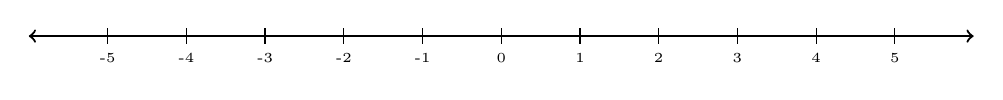
\begin{tikzpicture}
                \draw[<->,thick] (-6,0) -- (6,0);
                \foreach \x in {-5,-4,-3,-2,-1,0,1,2,3,4,5}
                    \draw (\x,0.1) -- (\x,-0.1) node[below] {\tiny\x};
            \end{tikzpicture}
            \end{center}

            \vspace{0.5cm}

            \textbf{(b)} Write the solution in interval notation.

            \vspace{2cm}

            \textbf{Problem 10}\\\\
            Solve: $-5 < 2x + 1 \leq 7$

            \vspace{3cm}

            \textbf{(a)} Graph the solution on a number line.

            \vspace{0.5cm}

            \begin{center}
            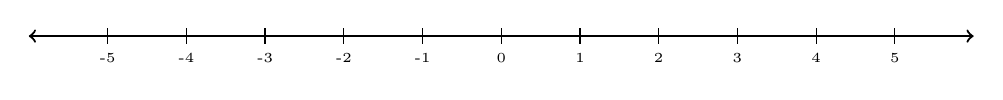
\begin{tikzpicture}
                \draw[<->,thick] (-6,0) -- (6,0);
                \foreach \x in {-5,-4,-3,-2,-1,0,1,2,3,4,5}
                    \draw (\x,0.1) -- (\x,-0.1) node[below] {\tiny\x};
            \end{tikzpicture}
            \end{center}

            \vspace{0.5cm}

            \textbf{(b)} Write the solution in interval notation.

            \newpage

            \textbf{Problem 11}\\\\
            A streaming service costs \$8.99 per month.\\\\
            You have a \$50 gift card.\\\\
            Write and solve an inequality to find the maximum number of whole months you can subscribe.

            \newpage

        \section*{Part D: Linear Functions \& Lines}

            \textbf{Problem 12}\\\\
            Find the slope of the line through $(3, -2)$ and $(-1, 6)$.

            \vspace{3cm}

            \textbf{Problem 13}\\\\
            Write the equation of a line with slope $-\displaystyle\frac{2}{3}$ and $y$-intercept 4.

            \vspace{3cm}

            \textbf{Problem 14}\\\\
            Convert to slope-intercept form: $3x - 4y = 24$\\\\
            State $m$ and $b$.

            \vspace{3cm}

            \textbf{Problem 15}\\\\
            Find the equation of the line through the points $(1, 7)$ and $(4, -2)$.

            \newpage

        \section*{Solutions}

            \subsection*{Part A: Foundations (Order of Operations \& Properties)}

            \textbf{Problem 1}\\\\
            Simplify: $8 + 12 \div 4 - 2 \times 3$

            \textit{Solution:}\\
            Follow PEMDAS (division and multiplication before addition and subtraction):\\
            $8 + 12 \div 4 - 2 \times 3$\\
            $= 8 + 3 - 6$\\
            $= 11 - 6$\\
            $= 5$

            \fbox{Answer: 5}

            \vspace{0.5cm}

            \textbf{Problem 2}\\\\
            Simplify: $(15 - 3)^2 \div 6 + 4$

            \textit{Solution:}\\
            Follow PEMDAS (parentheses first, then exponents, then division, then addition):\\
            $(15 - 3)^2 \div 6 + 4$\\
            $= (12)^2 \div 6 + 4$\\
            $= 144 \div 6 + 4$\\
            $= 24 + 4$\\
            $= 28$

            \fbox{Answer: 28}

            \vspace{0.5cm}

            \textbf{Problem 3}\\\\
            Simplify by combining like terms: $8x - 3y + 2x + 7y - 5$

            \textit{Solution:}\\
            Combine like terms (group $x$ terms, $y$ terms, and constants):\\
            $8x - 3y + 2x + 7y - 5$\\
            $= (8x + 2x) + (-3y + 7y) - 5$\\
            $= 10x + 4y - 5$

            \fbox{Answer: $10x + 4y - 5$}

            \newpage

            \textbf{Problem 4}\\\\
            Simplify: $4(2x - 3) - 3(x + 5) + 7$

            \textit{Solution:}\\
            Use the distributive property, then combine like terms:\\
            $4(2x - 3) - 3(x + 5) + 7$\\
            $= 8x - 12 - 3x - 15 + 7$\\
            $= (8x - 3x) + (-12 - 15 + 7)$\\
            $= 5x - 20$

            \fbox{Answer: $5x - 20$}

            \vspace{0.5cm}

            \textbf{Problem 5}\\\\
            A rectangular garden has length $(3x + 5)$ feet and width $(2x - 1)$ feet.\\
            Write a simplified expression for the perimeter.

            \textit{Solution:}\\
            Perimeter = $2(\text{length}) + 2(\text{width})$\\
            $P = 2(3x + 5) + 2(2x - 1)$\\
            $= 6x + 10 + 4x - 2$\\
            $= 10x + 8$

            \fbox{Answer: $(10x + 8)$ feet}

            \newpage

            \subsection*{Part B: Equations}

            \textbf{Problem 6}\\\\
            Solve: $5x - 8 = 2x + 13$

            \textit{Solution:}\\
            $5x - 8 = 2x + 13$\\
            $5x - 2x = 13 + 8$ \quad (subtract $2x$ from both sides, add 8 to both sides)\\
            $3x = 21$\\
            $x = 7$ \quad (divide both sides by 3)

            \fbox{Answer: $x = 7$}

            \vspace{0.5cm}

            \textbf{Problem 7}\\\\
            Solve: $\displaystyle\frac{1}{3}(x - 6) = 0.5x + 4$

            \textit{Solution:}\\
            Multiply both sides by 6 to clear fractions (LCD of 3 and 2):\\
            $6 \cdot \displaystyle\frac{1}{3}(x - 6) = 6(0.5x + 4)$\\
            $2(x - 6) = 3x + 24$\\
            $2x - 12 = 3x + 24$\\
            $-12 - 24 = 3x - 2x$\\
            $-36 = x$

            \fbox{Answer: $x = -36$}

            \vspace{0.5cm}

            \textbf{Problem 8}\\\\
            Solve for $h$: $\displaystyle A = \frac{1}{2}bh$

            \textit{Solution:}\\
            Multiply both sides by 2:\\
            $2A = bh$\\
            Divide both sides by $b$:\\
            $\displaystyle\frac{2A}{b} = h$

            \fbox{Answer: $h = \displaystyle\frac{2A}{b}$}

            \newpage

            \subsection*{Part C: Inequalities}

            \textbf{Problem 9}\\\\
            Solve: $-4x + 7 \leq -9$

            \textit{Solution:}\\
            $-4x + 7 \leq -9$\\
            $-4x \leq -16$ \quad (subtract 7 from both sides)\\
            $x \geq 4$ \quad (divide by $-4$; reverse inequality sign)

            \fbox{Answer: $x \geq 4$}

            \textbf{(a)} Graph the solution on a number line.

            \begin{center}
            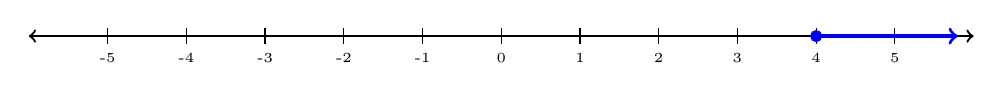
\begin{tikzpicture}
                \draw[<->,thick] (-6,0) -- (6,0);
                \foreach \x in {-5,-4,-3,-2,-1,0,1,2,3,4,5}
                    \draw (\x,0.1) -- (\x,-0.1) node[below] {\tiny\x};
                \draw[very thick, blue, ->] (4,0) -- (5.8,0);
                \filldraw[blue] (4,0) circle (2pt);
            \end{tikzpicture}
            \end{center}

            \textbf{(b)} Write the solution in interval notation.

            \fbox{Answer: $[4, \infty)$}

            \vspace{0.5cm}

            \textbf{Problem 10}\\\\
            Solve: $-5 < 2x + 1 \leq 7$

            \textit{Solution:}\\
            Solve the compound inequality by working on all parts:\\
            $-5 < 2x + 1 \leq 7$\\
            $-6 < 2x \leq 6$ \quad (subtract 1 from all parts)\\
            $-3 < x \leq 3$ \quad (divide all parts by 2)

            \fbox{Answer: $-3 < x \leq 3$}

            \textbf{(a)} Graph the solution on a number line.

            \begin{center}
            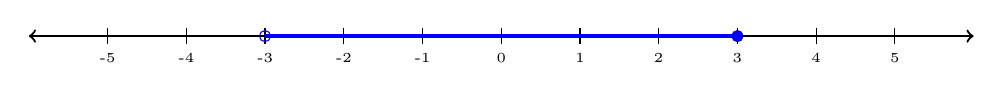
\begin{tikzpicture}
                \draw[<->,thick] (-6,0) -- (6,0);
                \foreach \x in {-5,-4,-3,-2,-1,0,1,2,3,4,5}
                    \draw (\x,0.1) -- (\x,-0.1) node[below] {\tiny\x};
                \draw[very thick, blue] (-3,0) -- (3,0);
                \draw[blue] (-3,0) circle (2pt);
                \filldraw[blue] (3,0) circle (2pt);
            \end{tikzpicture}
            \end{center}

            \textbf{(b)} Write the solution in interval notation.

            \fbox{Answer: $(-3, 3]$}

            \newpage

            \textbf{Problem 11}\\\\
            A streaming service costs \$8.99 per month. You have a \$50 gift card.\\
            Write and solve an inequality to find the maximum number of whole months you can subscribe.

            \textit{Solution:}\\
            Let $m$ = number of months\\
            The total cost must be less than or equal to \$50:\\
            $8.99m \leq 50$\\
            $m \leq \displaystyle\frac{50}{8.99}$\\
            $m \leq 5.56...$\\
            Since we need whole months: $m \leq 5$

            \fbox{Answer: Maximum of 5 months}

            \newpage

            \subsection*{Part D: Linear Functions \& Lines}

            \textbf{Problem 12}\\\\
            Find the slope of the line through $(3, -2)$ and $(-1, 6)$.

            \textit{Solution:}\\
            Use the slope formula: $m = \displaystyle\frac{y_2 - y_1}{x_2 - x_1}$\\
            $m = \displaystyle\frac{6 - (-2)}{-1 - 3}$\\
            $m = \displaystyle\frac{8}{-4}$\\
            $m = -2$

            \fbox{Answer: $m = -2$}

            \vspace{0.5cm}

            \textbf{Problem 13}\\\\
            Write the equation of a line with slope $-\displaystyle\frac{2}{3}$ and $y$-intercept 4.

            \textit{Solution:}\\
            Use slope-intercept form: $y = mx + b$\\
            Given: $m = -\displaystyle\frac{2}{3}$ and $b = 4$\\
            Substitute: $y = -\displaystyle\frac{2}{3}x + 4$

            \fbox{Answer: $y = -\displaystyle\frac{2}{3}x + 4$}

            \vspace{0.5cm}

            \textbf{Problem 14}\\\\
            Convert to slope-intercept form: $3x - 4y = 24$\\
            State $m$ and $b$.

            \textit{Solution:}\\
            Solve for $y$:\\
            $3x - 4y = 24$\\
            $-4y = -3x + 24$ \quad (subtract $3x$ from both sides)\\
            $y = \displaystyle\frac{3}{4}x - 6$ \quad (divide by $-4$)

            \fbox{Answer: $y = \displaystyle\frac{3}{4}x - 6$; $m = \displaystyle\frac{3}{4}$, $b = -6$}

            \newpage

            \textbf{Problem 15}\\\\
            Find the equation of the line through the points $(1, 7)$ and $(4, -2)$.

            \textit{Solution:}\\
            First find the slope:\\
            $m = \displaystyle\frac{-2 - 7}{4 - 1} = \frac{-9}{3} = -3$\\
            \\
            Use point-slope form with point $(1, 7)$:\\
            $y - 7 = -3(x - 1)$\\
            $y - 7 = -3x + 3$\\
            $y = -3x + 10$

            \fbox{Answer: $y = -3x + 10$}

\end{document}